
\subsubsection{Perceptrons}
Die simpelste Form eines Neuralen Netzwerks ist ein Perceptron. Es kann nur binäre Entscheidungen \{-1,+1\} treffen. Ein Perceptron besteht aus einer Input Layer und einem Output Node.
Die Input Layer beinhaltet $d$ nodes welches $d$ Merkmale $\overline{X} = [x_1...x_d]$ mit Weights $\overline{W} = [w_1...w_d]$ übermittelt. Die lineare Aktivierungsfunktion sign berechnet
dann die Vorhersage $\hat{y}$. \cite{CA18}\\
$$\hat{y} = sign\{\overline{W} \cdot \overline{X}\} = sign\{\sum\limits^{d}_{j=1}w_jx_j\}$$\\
In vielen Fällen wird ein nicht variables Element $b$ mit in der Rechnung berücksichtigt. Dies verursacht das der Mittelwert der Vorhersage nicht 0 ist. \cite{CA18}\\
$$\hat{y} = sign\{\overline{W} \cdot \overline{X} + b\} = sign\{\sum\limits^{d}_{j=1}w_jx_j + b\}$$\\
\begin{figure}[H]
    \begin{subfigure}{0.5\textwidth}
        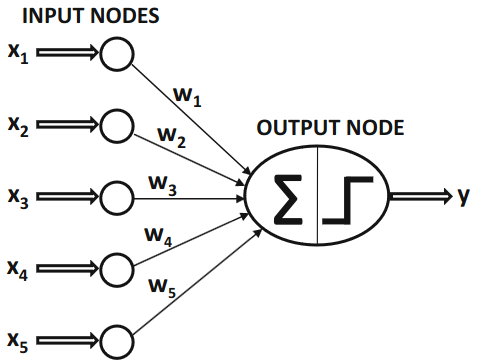
\includegraphics[width=\textwidth]{Sources/02-01_perceptron.png}
        \label{Synapse}
        \caption{{Perceptron ohne Bias}}
    \end{subfigure}
    \begin{subfigure}{0.5\textwidth}
        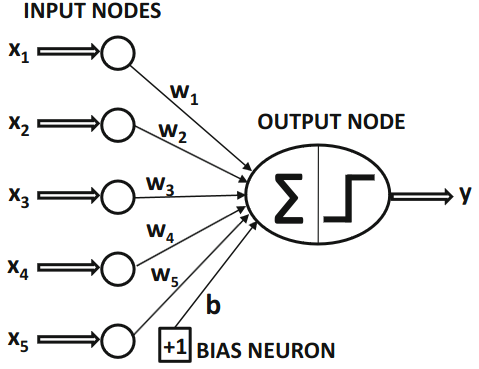
\includegraphics[width=\textwidth]{Sources/02-02_perceptronMitBias.png}
        \label{Neuron}
        \caption{Perceptron mit Bias}
    \end{subfigure}
    \caption{Aufbau von Perceptronen, Bild aus dem Buch 'Neural Networks and Deep Learning' von Charu C. Aggarwal
    }
    \end{figure}

\noindent 
Durch der so genannten Minimierung lässt sich der Fehler der Vorhersage verringern. Hierzu werden neben den Features x, auch Labels y in einem Feature-Label Paar eingeführt. 
$$\text{Minimize}_{\overline{W}}L = \sum\limits_{(\overline{X},y)\in \mathcal{D}}(y - \hat{y})^2 = \sum\limits_{(\overline{X},y)\in \mathcal{D}}(y - sign\{\overline{W} \cdot \overline{X}\})^2$$
Diese Art der Minimierung wird auch als Loss-Funktion bezeichnet. Die obige Funktion führt zu einer treppenstufigen Loss-Ebene, welche für gradient-descent ungeignet ist. Um diesem Problem entgegen zu wirken, wird eine Smooth-Funktion angewendet.
$$\Delta L_{\text{smooth}} = \sum\limits_{(\overline{X},y)\in \mathcal{D}}(y - \hat{y})\overline{X}$$
Beim Trainieren eines Neuralen Netzwerks werden Eingabedaten $\overline{X}$ einzelt oder in kleinen Batches eingespeist um die Vorhersage $\hat{y}$ zu generieren. Die Weights werden dann durch den Fehlerwert $E(\overline{X}) = (y - \hat{y})$ aktualisiert.
$$\overline{W} \Rightarrow \overline{W} + \alpha(y - \hat{y})\overline{X}$$
Der Parameter $\alpha$ reguliert die Lernrate des Neuralen Netzwerks. Der Perceptron-Algorithmus durchläuft die Trainingsdaten mehrmals bis die Weight-Werte konvergieren. Ein solcher Durchlauf wird als Epoche bezeichnet.\\
Der Perceptron-Algorithmus kann auch als stochastische Gradientenabstiegsmethode betrachtet werden. \cite{CA18}